\documentclass[tikz,border=12pt]{standalone}
\usepackage[T1]{fontenc}
\usepackage{mathpazo}
\usepackage{amsmath,amssymb}
\usetikzlibrary{arrows.meta, calc}

\definecolor{stblue}{HTML}{7B97AD}
\definecolor{rwgold}{HTML}{B8995E}
\definecolor{sage}{HTML}{7A9A7E}
\definecolor{dkbrown}{HTML}{3D3530}
\definecolor{wmgray}{HTML}{7B7067}
\definecolor{cream}{HTML}{F9F6F0}
\definecolor{border}{HTML}{D4C9B8}
\definecolor{terracotta}{HTML}{C47A6A}
\definecolor{lavender}{HTML}{907EA0}

\begin{document}
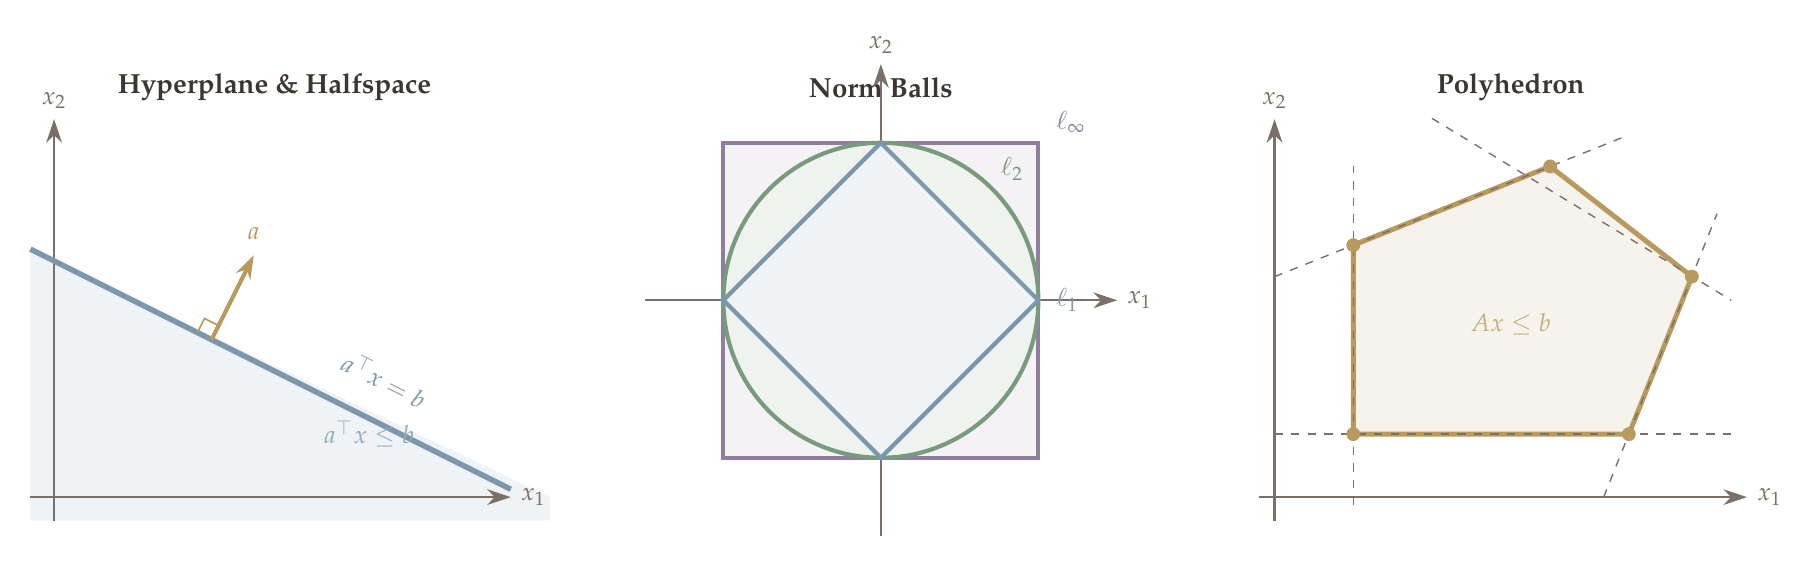
\begin{tikzpicture}[>={Stealth[length=3mm, width=2mm]}]

% ============================================================
% Panel 1: Hyperplane and Halfspace
% Line: x1 + 2*x2 = 6, from (0,3) to (6,0)
% Normal a = (1,2)/sqrt(5), pointing away from halfspace
% ============================================================
\node[font=\normalsize\bfseries, text=dkbrown] at (2.8,5.2) {Hyperplane \& Halfspace};

% Halfspace shading: x1 + 2*x2 <= 6 (below/left of the line)
\fill[stblue!12] (-0.3,-0.3) -- (-0.3,3.15) -- (6.3,0) -- (6.3,-0.3) -- cycle;

% Axes
\draw[wmgray, ->, line width=0.8pt] (-0.3,0) -- (5.8,0) node[right, font=\small] {$x_1$};
\draw[wmgray, ->, line width=0.8pt] (0,-0.3) -- (0,4.8) node[above, font=\small] {$x_2$};

% Hyperplane line
\draw[stblue, line width=2pt] (-0.3,3.15) -- (5.8,0.1);
\node[stblue, font=\small, rotate=-26.57] at (4.2,1.5) {$a^\top x = b$};

% Normal vector at (2,2), perpendicular: direction (1,2)/sqrt(5), length 1.2
% Endpoint: (2+1.2*0.4472, 2+1.2*0.8944) = (2.537, 3.073)
\draw[rwgold, ->, line width=1.5pt] (2,2) -- (2.537,3.073);
\node[rwgold, font=\small, anchor=south] at (2.537,3.15) {$a$};

% Right-angle mark (size 0.2)
% Along-line dir: (-2,1)/sqrt(5) = (-0.894,0.447)
% Normal dir: (1,2)/sqrt(5) = (0.447,0.894)
\draw[rwgold, line width=0.6pt]
  (1.821,2.089) -- (1.911,2.268) -- (2.089,2.179);

% Halfspace label
\node[stblue!80, font=\small] at (4,0.8) {$a^\top x \leq b$};

% ============================================================
% Panel 2: Norm Balls (all centered at origin, radius 2)
% ============================================================
\node[font=\normalsize\bfseries, text=dkbrown] at (10.5,5.2) {Norm Balls};

% Axes through center (10.5, 2.5)
\draw[wmgray, ->, line width=0.8pt] (7.5,2.5) -- (13.5,2.5) node[right, font=\small] {$x_1$};
\draw[wmgray, ->, line width=0.8pt] (10.5,-0.5) -- (10.5,5.5) node[above, font=\small] {$x_2$};

% L-infinity ball (square, radius 2)
\fill[lavender!10] (8.5,0.5) rectangle (12.5,4.5);
\draw[lavender, line width=1.5pt] (8.5,0.5) rectangle (12.5,4.5);

% L2 ball (circle, radius 2)
\fill[sage!12] (10.5,2.5) circle (2);
\draw[sage, line width=1.5pt] (10.5,2.5) circle (2);

% L1 ball (diamond, radius 2)
\fill[stblue!12] (10.5,4.5) -- (12.5,2.5) -- (10.5,0.5) -- (8.5,2.5) -- cycle;
\draw[stblue, line width=1.5pt] (10.5,4.5) -- (12.5,2.5) -- (10.5,0.5) -- (8.5,2.5) -- cycle;

% Labels
\node[lavender, font=\small, anchor=south west] at (12.6,4.5) {$\ell_\infty$};
\node[sage, font=\small, anchor=south west] at (11.9,3.9) {$\ell_2$};
\node[stblue, font=\small, anchor=west] at (12.6,2.5) {$\ell_1$};

% ============================================================
% Panel 3: Polyhedron (intersection of halfspaces)
% ============================================================
\node[font=\normalsize\bfseries, text=dkbrown] at (18.5,5.2) {Polyhedron};

% Axes
\draw[wmgray, ->, line width=0.8pt] (15.3,0) -- (21.5,0) node[right, font=\small] {$x_1$};
\draw[wmgray, ->, line width=0.8pt] (15.5,-0.3) -- (15.5,4.8) node[above, font=\small] {$x_2$};

% Polyhedron vertices
\coordinate (v1) at (16.5,0.8);
\coordinate (v2) at (20,0.8);
\coordinate (v3) at (20.8,2.8);
\coordinate (v4) at (19,4.2);
\coordinate (v5) at (16.5,3.2);

% Fill and draw polygon
\fill[rwgold!12] (v1) -- (v2) -- (v3) -- (v4) -- (v5) -- cycle;
\draw[rwgold, line width=1.8pt] (v1) -- (v2) -- (v3) -- (v4) -- (v5) -- cycle;

% Edge extensions (dashed) — each extends the corresponding polygon edge
% Edge 1: v1--v2, y=0.8 horizontal
\draw[wmgray, line width=0.5pt, dashed] (15.5,0.8) -- (21.3,0.8);
% Edge 2: v2--v3, slope=(2.8-0.8)/(20.8-20)=2.5
\draw[wmgray, line width=0.5pt, dashed] (19.68,0) -- (21.12,3.6);
% Edge 3: v3--v4, slope=(4.2-2.8)/(19-20.8)=-0.609
\draw[wmgray, line width=0.5pt, dashed] (17.5,4.81) -- (21.3,2.50);
% Edge 4: v4--v5, slope=(3.2-4.2)/(16.5-19)=0.4
\draw[wmgray, line width=0.5pt, dashed] (15.5,2.8) -- (20,4.6);
% Edge 5: v5--v1, x=16.5 vertical
\draw[wmgray, line width=0.5pt, dashed] (16.5,-0.1) -- (16.5,4.2);

% Vertex dots
\foreach \v in {v1, v2, v3, v4, v5} {
  \fill[rwgold] (\v) circle (2.5pt);
}

% Label
\node[rwgold!80, font=\small] at (18.5,2.2) {$Ax \leq b$};

\end{tikzpicture}
\end{document}
